\subsection{Proof Generation}\label{section: zk-zkvm-user-end-prove}

Sections \ref{section: zk-zkvm-keys-addresses} and \ref{section: zk-zkvm-notes} serve as core building blocks of our ZK-ZKVM system. In this section, we will explain our proof generation scheme. For a high-level overview of the system design, please refer to section \ref{section: zk-zkvm-framework}.

Proof generation is a critical component of the ZK-ZKVM platform, designed to facilitate private and efficient execution of smart contracts on the blockchain. The platform offers both public and private functions, with private functions executed and proven on the user-side, while public functions are executed and verified on blockchain nodes.

To enable this functionality, ZK-ZKVM relies on advanced cryptographic techniques such as the key system discussed in section \ref{section: zk-zkvm-keys-addresses} and note design discussed in section \ref{section: zk-zkvm-notes}. These tools allow users to generate compact and efficient proofs that demonstrate their authorization to execute private functions without revealing any sensitive information about those functions.

The proof generation process involves several steps. First, in a single contract function call, there may be private and public functions. The user executes and generates a set of data (including private and public inputs) for the private function, along with a callback hook for the public function. They then use this data to generate a zero-knowledge proof that demonstrates their authorization to execute the function and validates the execution.

Next, the user submits this proof, along with their public inputs, to the blockchain node for verification. The node verifies the proof using ZK-ZKVM's public parameters (referred to as the verification key in ZK-SNARKs) to ensure that the private function is executed correctly.

Once the proof is verified, the network executes any relevant public functions on behalf of the user with the provided callback hook. Throughout this process, all sensitive information about the private function remains hidden from public view, ensuring strong privacy guarantees for all parties involved. Public state information, such as Note Commitments Tree and Nullifier Set, is stored on the node side and public functions are handled on the node as well.

\textbf{\large Procedure.} A Transaction is constructed as Fig\ref{fig:transaction_construction}:
\begin{figure}[!ht]
    \centering
    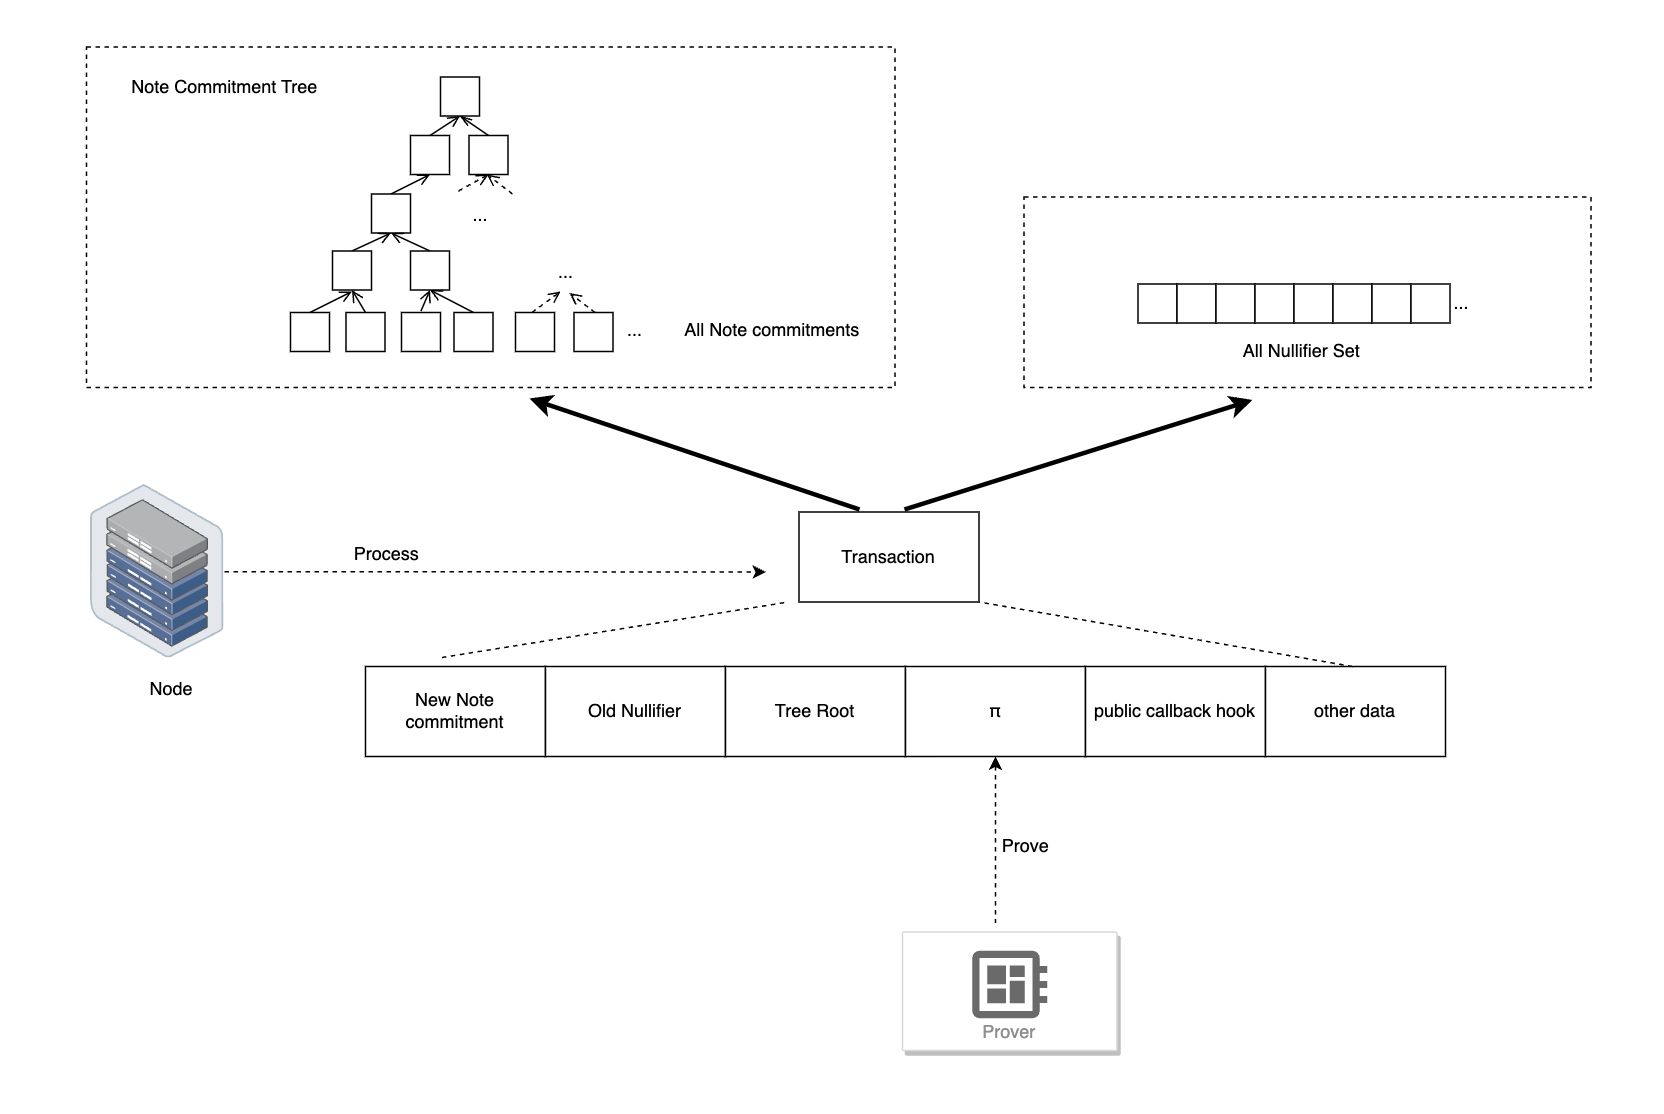
\includegraphics[width=0.6\textwidth]{Transaction construction.jpg}
    \caption{Transaction construction}
    \label{fig:transaction_construction}
\end{figure}

As previously mentioned, proving the value of $\pi$ is a crucial aspect of our transaction. Therefore, this section will primarily focus on the generation of proofs. Below are several critical proof statements, which, although brief, hold great significance:

\color{blue!50!black}
\begin{obeylines}
$\exists$   old Notes ($Note_{old,1}, Note_{old,2}, ..., Note_{old,n}$)
    old secret keys ($ask_{old,1}, ask_{old,2}, ..., ask_{old,n}$)
    new Notes ($Note_{new,1}, Note_{new,2}, ..., Note_{new,m}$)
    other auxiliary input $aux$
\textbf{such that:}
    each old note $Note_{old,i}$:
    \begin{itemize}
        \item[-] has a commitment that is in note commitments tree with tree root $R_L$.
        \item[-] is owned by secret key $ask_{old,i}$
        \item[-] has a nullifier $nf_i$ 
    \end{itemize}
    each new note $Note_{new,i}$ has commitment $cm_j$, and new commitment is unique.
\end{obeylines}

\normalcolor{}

When all the required parts match, including any other necessary components, the prover is able to produce a valid proof $\pi$ for the transaction.

Here is a more detailed explanation proof generation phase:
\color{blue!50!black}

\textbf{Input:}

\begin{itemize}
    \item public parameters $pp$
    \item old  \[ \begin{cases} \text{notes $[n_i]_1^n$} \\ \text{address secret keys $[ask_i]_1^n$} \end{cases} \]
    \item new \[
        \begin{cases} \text{address public keys $[apk_j]_1^m$} \\ \text{note payload $[payload_i]_1^m$} \\
            \text{note birth predicates $[\Phi_{b,j}]_1^m$} \\ \text{note death predicates $[\Phi_{d,j}]_1^m$}
        \end{cases}
        \]
    \item auxiliary predicate input $aux$
    \item transaction memorandum $memo$
\end{itemize}

\textbf{Output:} new notes $[n_j]_1^m$ and transaction tx that contains public function callback hooks $[hook_j]_1^m$ (if public functions are called)

\begin{enumerate}
    \item For each $i \in \{1, ..., n\}$, process the $i$-th old note as follows:
        \begin{enumerate}
            \item Parse old note $n_i$ as $(apk_i, payload_i, \rho, predicates(\Phi_{b,i}, \Phi_{d,i}), commitment \ cm_i)$
            \item Compute \textbf{Note Commitments Tree(NCT) membership witness} for commitment: $W_{L,i} \leftarrow NCT.Prove(cm_i)$
            \item Compute \textbf{nullifier number:} $nf_i \leftarrow PRF(\rho)$
        \end{enumerate}
    \item For each $j \in \{1, ..., m\}$, construct the $j$-th new note as follows:
        \begin{enumerate}
            \item Compute \textbf{nullifier nonce:} $\rho_j := Hash(pp_{CRH} || nf_1 || ... || nf_n)$
            \item Construct \textbf{new note:} $cm_j \leftarrow ConstructNote(apk_j, payload_j, \Phi_{b,j}, \Phi_{d,j}, \rho_j)$
        \end{enumerate}
    \item Retrieve current Note Commitments Tree root: $R_L \leftarrow NCT.Root$.
    \item Construct instance $X_e$ for curcuit: $X_e := (R_L, [nf_i]_1^n, [cm_j]_1^m, memo, [hook_j]_1^m)$
    \item Construct witness $W_e$ for circuit: $W_e := ([n_i]_1^n, [W_{L,i}]_1^n, [ask_i]_1^n, [n_j]_1^m, aux)$
    \item Generate \textbf{proof for:} $\pi \leftarrow Starky.Prove(pp, X_e, W_e)$
    \item Construct \textbf{transaction:} $tx := ([nf_j]_1^n, [cm_j]_1^m, memo, R_L, \pi, [hook_j]_1^m)$
    \item New notes and new constructed transaction: $([n_j]_1^m, tx)$
\end{enumerate}
\normalcolor{}

For additional information on the inner workings of Starky and how it produces proofs, please refer to this resource \ref{section: starky-zkvm}.